% Options for packages loaded elsewhere
\PassOptionsToPackage{unicode}{hyperref}
\PassOptionsToPackage{hyphens}{url}
%
\documentclass[
]{article}
\usepackage{amsmath,amssymb}
\usepackage{iftex}
\ifPDFTeX
  \usepackage[T1]{fontenc}
  \usepackage[utf8]{inputenc}
  \usepackage{textcomp} % provide euro and other symbols
\else % if luatex or xetex
  \usepackage{unicode-math} % this also loads fontspec
  \defaultfontfeatures{Scale=MatchLowercase}
  \defaultfontfeatures[\rmfamily]{Ligatures=TeX,Scale=1}
\fi
\usepackage{lmodern}
\ifPDFTeX\else
  % xetex/luatex font selection
\fi
% Use upquote if available, for straight quotes in verbatim environments
\IfFileExists{upquote.sty}{\usepackage{upquote}}{}
\IfFileExists{microtype.sty}{% use microtype if available
  \usepackage[]{microtype}
  \UseMicrotypeSet[protrusion]{basicmath} % disable protrusion for tt fonts
}{}
\makeatletter
\@ifundefined{KOMAClassName}{% if non-KOMA class
  \IfFileExists{parskip.sty}{%
    \usepackage{parskip}
  }{% else
    \setlength{\parindent}{0pt}
    \setlength{\parskip}{6pt plus 2pt minus 1pt}}
}{% if KOMA class
  \KOMAoptions{parskip=half}}
\makeatother
\usepackage{xcolor}
\usepackage[margin=1in]{geometry}
\usepackage{graphicx}
\makeatletter
\def\maxwidth{\ifdim\Gin@nat@width>\linewidth\linewidth\else\Gin@nat@width\fi}
\def\maxheight{\ifdim\Gin@nat@height>\textheight\textheight\else\Gin@nat@height\fi}
\makeatother
% Scale images if necessary, so that they will not overflow the page
% margins by default, and it is still possible to overwrite the defaults
% using explicit options in \includegraphics[width, height, ...]{}
\setkeys{Gin}{width=\maxwidth,height=\maxheight,keepaspectratio}
% Set default figure placement to htbp
\makeatletter
\def\fps@figure{htbp}
\makeatother
\setlength{\emergencystretch}{3em} % prevent overfull lines
\providecommand{\tightlist}{%
  \setlength{\itemsep}{0pt}\setlength{\parskip}{0pt}}
\setcounter{secnumdepth}{-\maxdimen} % remove section numbering
\ifLuaTeX
  \usepackage{selnolig}  % disable illegal ligatures
\fi
\usepackage{bookmark}
\IfFileExists{xurl.sty}{\usepackage{xurl}}{} % add URL line breaks if available
\urlstyle{same}
\hypersetup{
  hidelinks,
  pdfcreator={LaTeX via pandoc}}

\author{}
\date{\vspace{-2.5em}}

\begin{document}

\section{Appendix i: Soundness of bootstrap resampling
procedure}\label{appendix-i-soundness-of-bootstrap-resampling-procedure}

We report here the results of simulations that indicate the soundness of
our bootstrapping procedure. We seek to determine that we have not
biased our results on the basis of our sampling method. These
simulations also justify the soundness of the analysis in Lorca-Puls et
al (2018). The code of these simulations is available at the online
repository for this study.

We assume a ``base-sample'', which in this paper would be the collection
of 313 participants that performed each of the four executive function
and implicit learning experiments. For Lorca-Puls et al (2018) it would
be a large set (360) of patients selected from the Ploras database
according to some criteria and for the simulations discussed here a
large set (360) of numbers sampled from a Gaussian. The key property we
are seeking to verify is the following: \emph{For a given
``base-sample'', sampling directly with replacement (direct\_wi\_rep)
from the base-sample generates the same uncertainty (i.e.~standard
deviations (stds)) as sampling indirectly with replacement
(indirect\_wi\_rep) from the base-sample} (see below for a definition of
indirect\_wi\_rep).

The simulations proceed as follows, using the sample sizes employed in
Lorca-Puls et al (2018), which are comparable to the current work.

\subsubsection{Basic procedure}\label{basic-procedure}

\begin{enumerate}
\def\labelenumi{\arabic{enumi}.}
\tightlist
\item
  Sample a base sample of size 360 from a gaussian, call this
  \emph{base-sample}.
\item
  Sample from base-sample to generate subsamples with sizes ranging from
  330 to 30 (in steps of 30), we denote these sizes with M. For all of
  these subsample sizes, N samples are taken. Thus, we are left with N
  samples all of size 330, N samples all of size 300, N samples all of
  size 270, and so on down to N samples all of size 30. (Conceptually,
  one of the N samples of a particular size represents the data that
  could have been collected in a single experiment with M participants.)
\item
  These subsamples were taken under four different sampling procedures:
\end{enumerate}

\begin{enumerate}
\def\labelenumi{\alph{enumi}.}
\item
  \emph{direct\_wi\_rep}: this is a bootstrapping procedure (hence,
  \emph{wi\_rep}, i.e.~with replacement), and the bootstrap samples are
  taken directly from the \emph{base-sample} (hence, \emph{direct}).
\item
  \emph{direct\_w/o\_rep}: this again samples directly from the
  base-sample, but it is not bootstrapping, since samples are taken
  without replacement; as a result, there is no duplication of elements
  within each sample, although different samples can include the same
  elements.
\item
  \emph{indirect\_wi\_rep}: this is a bootstrapping procedure, but it
  involves two levels of sampling; that is, a first sample is taken
  (without replacement) from the \emph{base-sample}, which we call the
  \emph{intermediate} sample, and then subsamples proper are
  bootstrapped from this \emph{intermediate} sample.
\item
  \emph{disjoint}: this involves performing disjoint splits of the
  base-sample; accordingly, the smallest samples that can be generated
  are of size 180 for a \emph{base-sample} of size 360.
\end{enumerate}

We also have a \emph{reference} condition, which is a ground truth and
involves sampling directly from a gaussian, rather than directly or
indirectly from a \emph{base-sample}.

\begin{enumerate}
\def\labelenumi{\arabic{enumi}.}
\setcounter{enumi}{3}
\tightlist
\item
  For any subsample size and sampling procedure, we proceed as follows,
\end{enumerate}

\begin{enumerate}
\def\labelenumi{\alph{enumi}.}
\item
  We will have N subsamples.
\item
  Calculate the Cohen's \(d\) (difference from zero) effect size of each
  of these N subsamples.
\item
  The resulting (N item) distribution of Cohen's \(d\)'s is playing the
  role of one of the distributions of effect sizes in the main body of
  this paper.
\item
  We then calculate the standard deviation of this distribution of
  Cohen's d's, which plays the role of the dispersion of one of these
  distributions of effect sizes. We call this the basic procedure
  standard deviation.
\end{enumerate}

We now iterate over this basic procedure in order to determine the
statistics (central tendency and dispersion) of the \emph{basic
procedure standard deviations}. Thus, we run the basic procedure many
times and calculate a mean estimate of the standard deviation of basic
procedure distributions. We also calculate the standard deviation across
these \emph{basic procedure standard deviations}, in order to understand
the variability in a single running of the basic procedure.

\subsection{Results}\label{results}

The results of our simulations are shown in Figures 1 and 2.

\begin{figure}
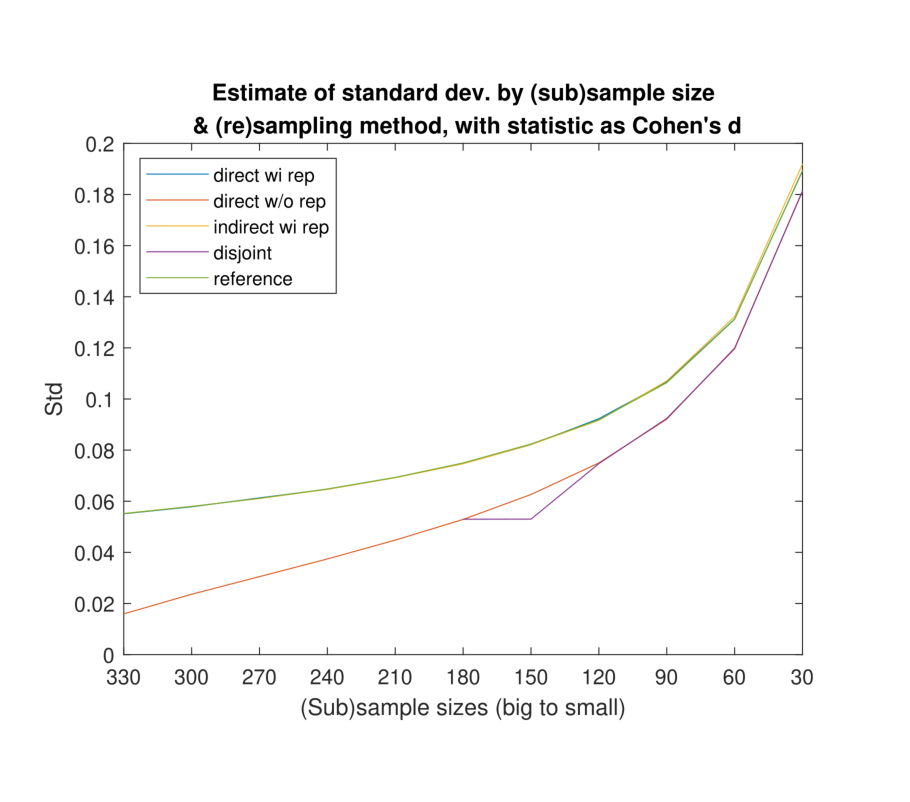
\includegraphics[width=0.7\linewidth]{figure1_sml} \caption{Figure 1: Mean estimate of basic procedure standard deviations, when the main statistic is the effect size. This corresponds to a central tendency estimate of the standard deviations of basic procedure distributions. This is given for a range of sub-sample sizes, and plotted for the four different resampling procedures, with the nature of the disjoint split procedure meaning that it cannot have subsample sizes greater than 180. The ground truth reference procedure is also shown. The lines for direct wi rep, indirect wi rep and reference, are sat on top of each other, while direct wo rep and disjoint, are sat on top of each other. Importantly, direct wi rep and indirect wi rep show the same pattern, which is our finding.}\label{fig:FigureSDs}
\end{figure}

Figure 1 is the main finding. Central tendencies are being estimated of
standard deviations of sets of parameter estimates (here, effect sizes),
each of which was generated from a resampling. So, this mirrors what
happens in the main body of this paper, where bootstrap samples are
generated, effect sizes of each are calculated and the results are put
into a distribution.

Critically, in figure 1, the \emph{direct\_wi\_rep} and
\emph{indirect\_wi\_rep} lines track each other. \emph{direct\_wi\_rep}
is the procedure employed in the main-body of this paper and Lorca-Puls
et al, i.e.~bootstrap smaller and smaller samples from single
(eventually much bigger) root data set (our \emph{base-sample}).
Consequently, the smaller samples will have less items in common between
samples, than the larger samples, and one might think this is what
causes the increased variability we see as samples get smaller, i.e.~the
increase in curves as one moves from left (large samples) to right
(small samples) in Figure 1.

The \emph{indirect\_wi\_rep} line counters this, since it first samples
an ``intermediate'' sample from the large, base, sample, which is the
size of the bootstrap samples then generated from it, e.g.~the
\emph{indirect\_wi\_rep} 60 data point is generated from bootstrap
samples of size 60 from a sample that was of size 60. Thus, at each
sample size, bootstrap samples were generated from samples of the same
size as the bootstrap samples.

Importantly, this does not change the pattern we observe of mean
estimates of standard deviations. An explanation of why the
\emph{indirect\_wi\_rep} curve is not different from the
\emph{direct\_wi\_rep} one is the following. Even if, on the
\emph{direct\_wi\_rep} curve, if you mapped subsamples to underlying
sets (mathematically, sets do not reflect repetition, just containing
each item that arises at least once) and then took the intersection, you
would find less overlap, as subsamples get smaller, that does not
automatically mean the procedure is invalid. That is, the variability in
bootstrapping is generated from the varying number of times (including
zero times) that the same items appear in a set. The combinatorics of
the variability generated in this way is so great that it swamps any
decreased overlap that would be apparent when going to underlying sets
(i.e.~removing repetitions). Indeed, this reflects what is the essential
property that makes bootstrapping work. For instance, when bootstrapping
samples of size R from a set of size R one will often generate bootstrap
samples where the underlying set of items in the samples is the same,
but the number of times each item appears in the bootstrap samples
varies; it is this variability in number of repetitions that creates the
variability in the statistic calculated using bootstrapping.

Our second set of findings are shown in Figure 2. Firstly, this shows
that all sampling procedures add uncertainty compared to the reference
procedure (which is our ground truth), and this effect increases with
reduction in subsample size. Thus, the sampling procedures create
variability, but (since the central tendency is accurate) not bias.

\begin{figure}
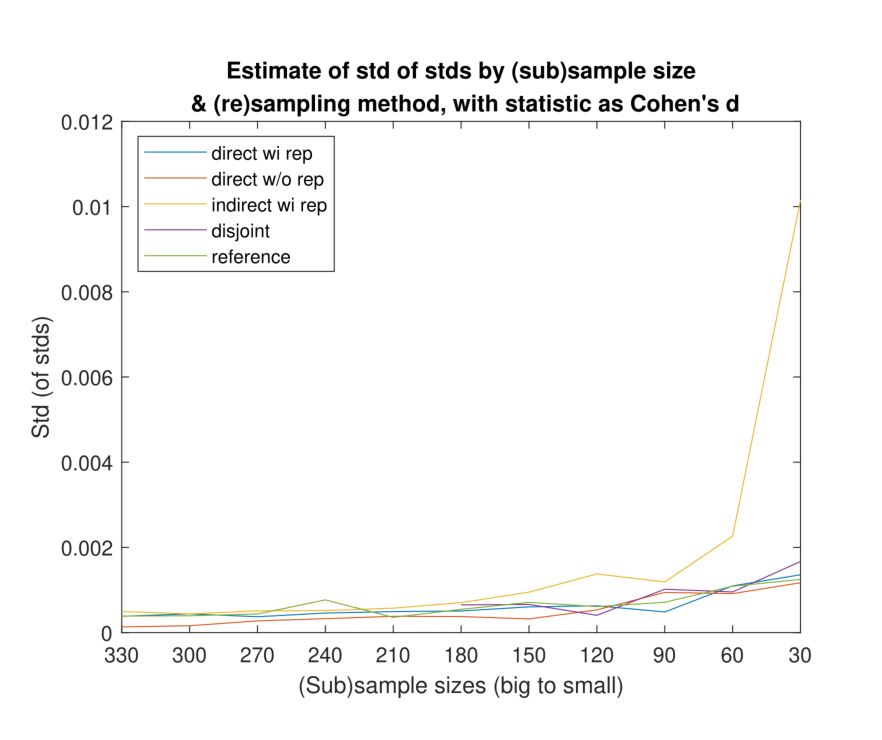
\includegraphics[width=0.7\linewidth]{figure2_sml} \caption{Estimate of standard deviation of basic procedure standard deviations, when the main statistic is the effect size. This corresponds to a dispersion estimate of the standard deviations of basic procedure distributions.  This is given for a range of sub-sample sizes. This is plotted for the four different resampling procedures, with the nature of the disjoint split procedure meaning that it cannot have subsample sizes greater than 180. The ground truth reference procedure is also shown. It is clear that indirect wi rep adds considerable variability to standard deviation estimates, as sample sizes get small.}\label{fig:FigureSDSDs}
\end{figure}

Further, Figure 2 shows that, while (as shown in Figure 1) the central
tendency across many repetitions (of the basic procedure) gives the same
dispersion estimate for \emph{indirect\_wi\_rep} and
\emph{direct\_wi\_rep}, the former is dramatically more variable in its
dispersion estimate than the latter. This then means that a single run
of the basic procedure, is likely to generate an inaccurate estimate of
the dispersion of a statistic if indirect\_wi\_rep is used. However,
since \emph{direct\_wi\_rep} exhibits the same central tendency for the
dispersion of the statistic, it can be used in place of
\emph{indirect\_wi\_rep}, with no loss and indeed, this is exactly what
is done in the main body of this paper and Lorca-Puls et al.~

This is important since, as previously discussed,
\emph{indirect\_wi\_rep} could be considered conceptually bullet-proof,
since the probability of overlap between subsamples does not reduce as
the sample size gets smaller.

The comparison of \emph{reference} and \emph{indirect\_wi\_rep} is also
of note. The point of interest for this appendix is what happens with
direct sampling with replacement (\emph{direct\_wi\_rep}) as the sample
size gets small, and whether there remains a non-trivial probability of
the same data points appearing in multiple samples even when the sample
size is small. This is because, it is the difference of this probability
of overlap between direct and indirect sampling that we are interested
in. Indeed, the most liberal test of our hypothesis (i.e.~giving the
greatest opportunity to find a disparity between direct and indirect
sampling) is one in which the probability of the same data points
appearing in multiple samples with direct sampling is vanishingly small.
This is what the \emph{reference} case gives us. With real numbers,
there is (mathematically) a probability of zero of sampling the same
number multiple times from a Gaussian, so all the samples generated
under \emph{reference} are disjoint by construction. (This is, of
course, putting aside issues of maximum precision available on a
particular computer, which no approach can overcome.) The fact that
\emph{reference} shows the same pattern as \emph{direct\_wi\_rep} in
Figures 1 and 2, suggests that increasing the size of the
\emph{base\_sample} in order to reduce sample overlap in
\emph{direct\_wi\_rep} will not change the basic findings, i.e.~what we
demonstrate here with base samples of 360 is in fact fully general.

\end{document}
